\section{Analisi del problema e Soluzioni}
In questa sezione verrà descritto il problema affrontato, le soluzioni scelte ed i rispettivi
risultati ottenuti.

\paragraph{Problema affrontato}
Il problema affrontato chiedeva di trovare pattern, anomalie e/o inferire sui dati forniti, 
per ottenere, come risultato, informazioni su di essi mediante l'utilizzo di tecniche 
dell'analisi di serie temporali, e quindi successivamente capire se quest'ultime possano essere 
utlizzate come tencniche ausiliarie per l'analisi a problemi di questa tipologia.

Per riuscire risolvere il problema posto e per questioni di tempo, il problema è stato 
ridotto all'analisi dei soli giunti del piede, più in particolare,
il tirocinio si è basato sulla ricerca di uno o più metodi utili a trovare la durata del passo
(stride) di un soggetto con una successiva analisi dei risultati.



\paragraph{Risultati attesi}
\begin{sloppypar}
Come risultato atteso è stata presa in considerazione l'eventualità della non riuscita dell'obbiettivo finale,
quindi l'impossibilità di trovare, tramite le tecniche dell'analisi di serie temporali, una possibile soluzione
al problema.
\end{sloppypar}

In caso positivo, quindi di una possibile soluzione al problema posto, i risultati attesi potrebbero essere:
\begin{itemize}
    \setlength\itemsep{-0.5em}
    \item Capacità da parte del metodo sviluppato di rilevare la durata del passo.
    \item Capacità da parte del metodo sviluppato di rilevare incorrettamente la durata del passo.
    \item Impossibilità da parte del metodo sviluppato di rilevare un passo.
\end{itemize}


\subsection{Prima soluzione}
In questa sezione verrà mostrata la prima soluzione al problema posto, nello specifico verrà
spiegata in breve l'idea generale, l'implementazione di alcuni dei metodi utilizzati, l'analisi dei
risultati, l'analisi della complessità ed infine le conclusioni.


\subsubsection{Idea generale}
L'idea generale, fulcro di questa soluzione, ruota intorno all'analisi della funzione di autocorrelazione.
Quest'ultima viene utilizzata per riconoscere pattern o una sorta di correlazione tra i dati non
visibile direttamente.

\subsubsection{Implementazione}
Come primo step implementativo è stato necessario scrivere una funzione che rendesse ogni serie stazionaria 
mediante l'ausilio del test di Dickey-Fuller ed il calcolo della prima differenza. Ovviamente
per rendere una serie stazionaria esistono anche altri metodi diversi dalla prima differenza ma 
si è deciso di utilizzarle quest'utlima per la sua semplicità.
\\
\paragraph*{Snippet} (\textit{Prima differenza})
\begin{minted}{python3}
    def compute_first_diff(series: list | np.ndarray):
        """ Calcola la prima differenza
        """
        
        if not isinstance(series, np.ndarray):
            series = np.array(series)

        return series[1:] - series[:len(series)-1]
\end{minted}

\paragraph*{Snippet} (\textit{Metodo per rendere la serie stazionaria})
\begin{minted}{python3}
    def make_stationary(series, max_steps = 30):
        """ Rende la serie stazionaria mediante il calcolo
            della prima differenza
        """
        step = 0   # numero di step
        s_copy = series.copy()  # copia della serie
        
        # fino a quando il test ritornca che la serie
        # non è stazionaria oppure sono stati superati
        # il massimo di step
        while(sts.adfuller(series)[1] > 0.05 
            and step < max_steps):
            
            # calcola la prima differenza
            serie = compute_first_diff(series)
            step += 1

        # se max_step è superato, non si è riusciti
        # a rendere la serie stazionaria
        if step > 30:
            series = s_copy

        return series
\end{minted}

\begin{sloppypar}
Dopo aver reso ogni serie stazionaria è stata applicata la funzione di autocorrelazione ad ognuna di
esse, per capire meglio i risultati di questa operazione prendiamo in cosniderazione alcuni dei 
grafici relativi all'autocorrelazione di serie appartenenti a dataset dei soggetti $6$ ed $12$.
\end{sloppypar}

\begin{figure}[H]
    \centering
    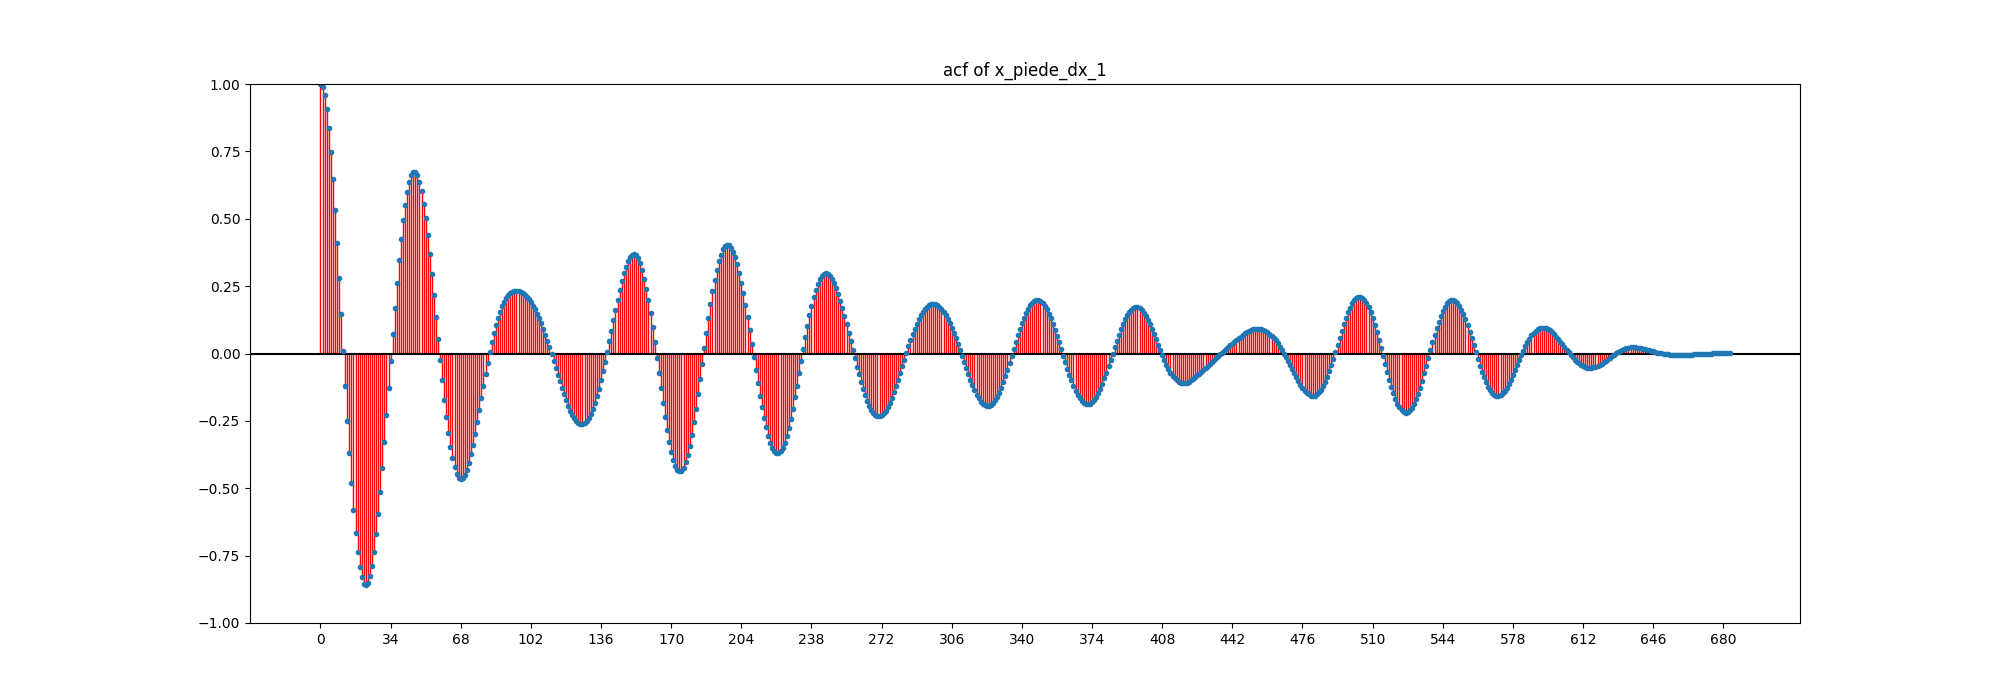
\includegraphics[width=\linewidth,keepaspectratio]{P006_x_piede_dx_1_acf.png}
    \caption{Soggetto $6$ autocorrelazione x piede destro posizione 1.}
    \label{fig:P006_x_piede_dx_1_acf}
\end{figure}

\begin{figure}[H]
    \centering
    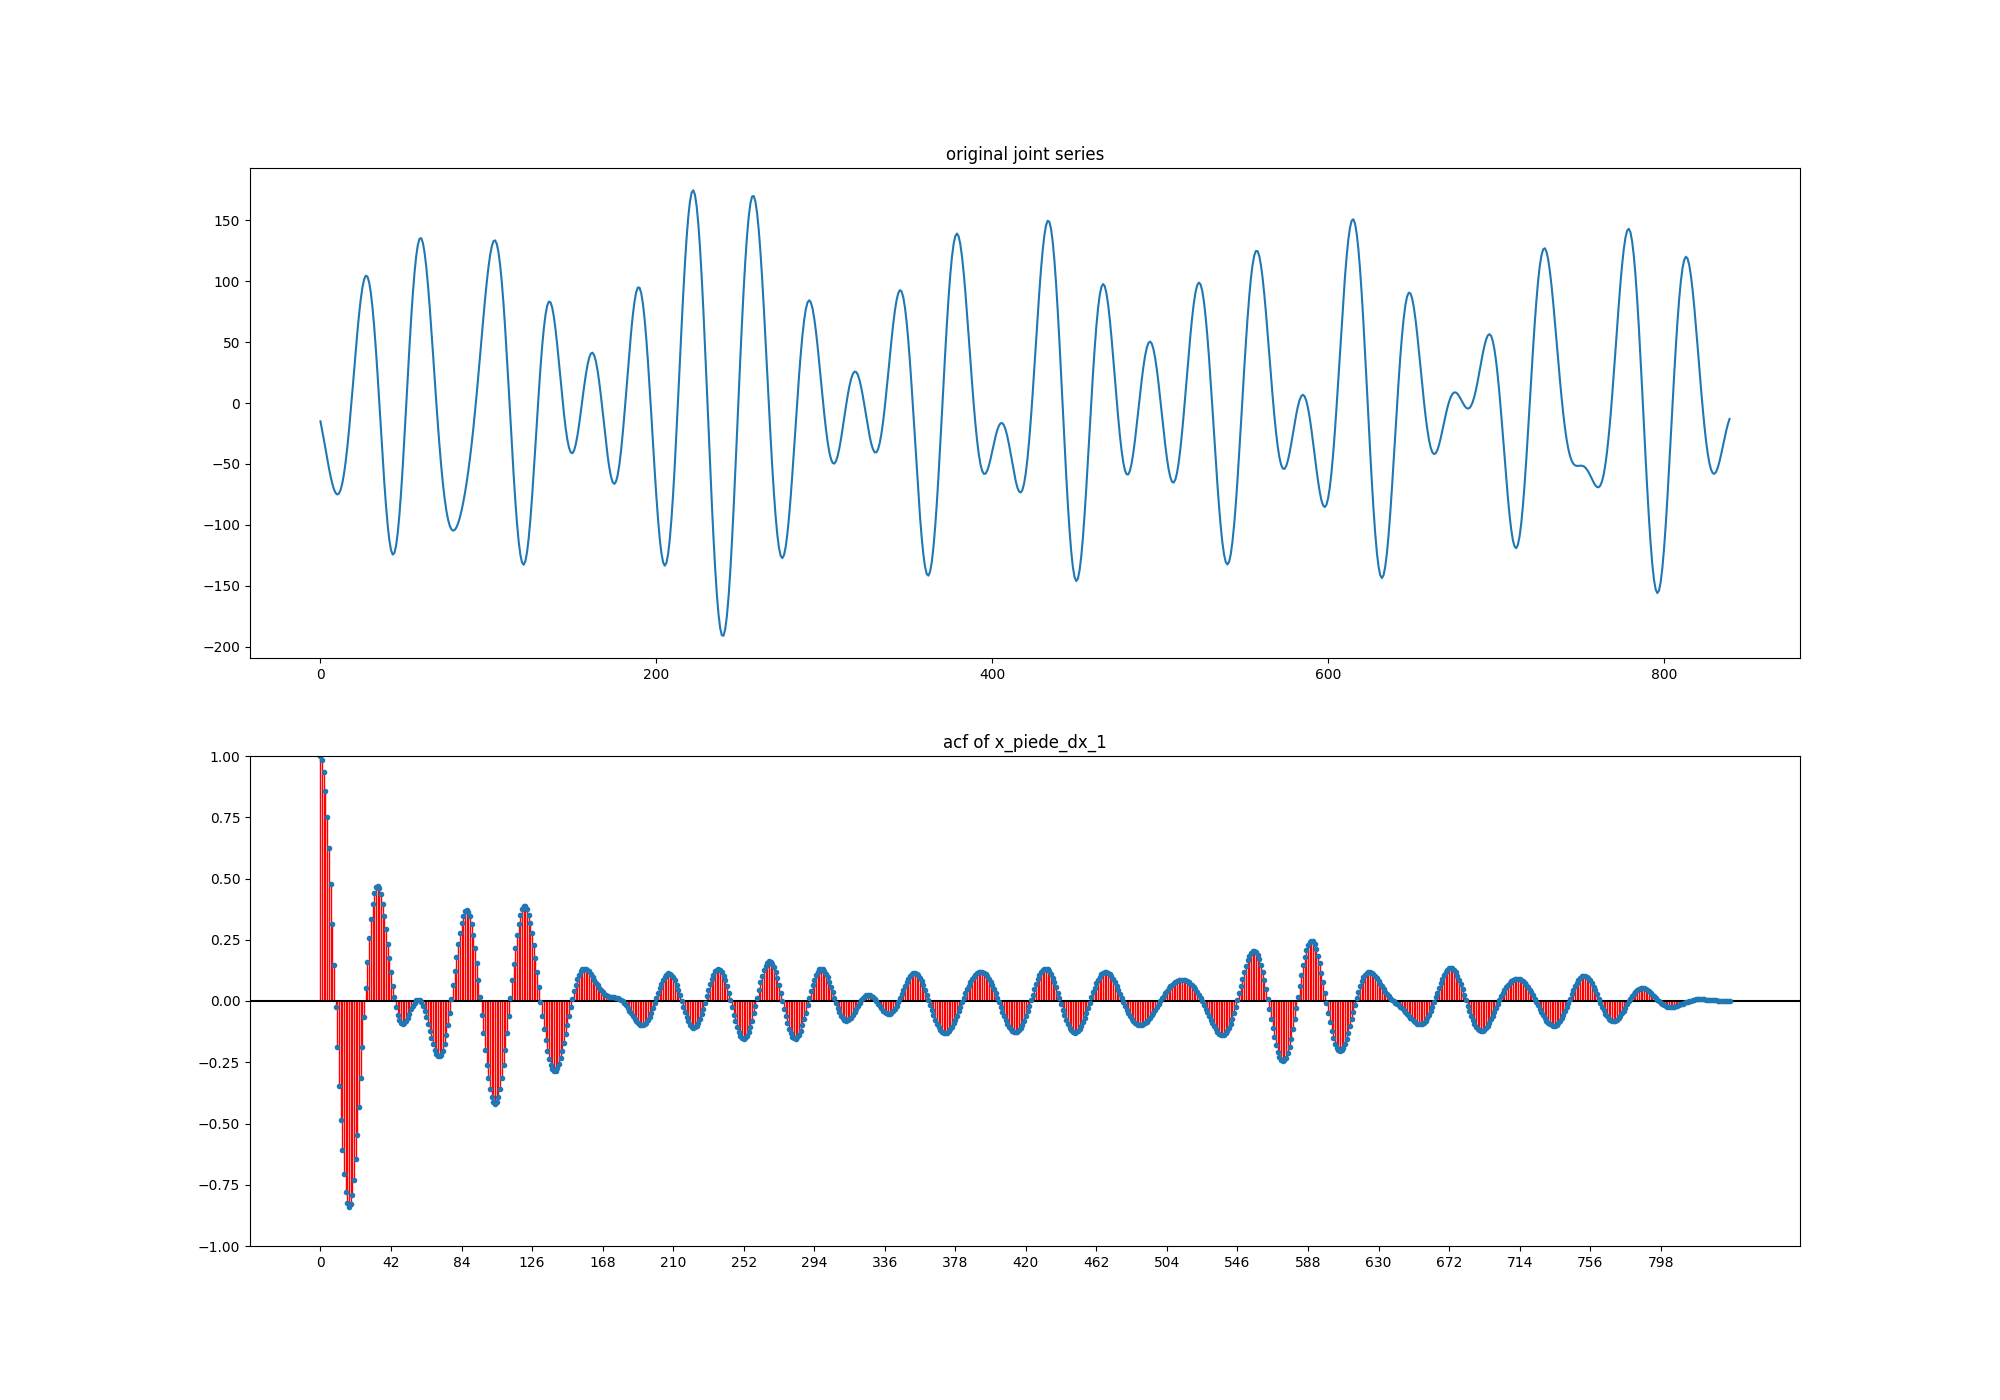
\includegraphics[width=\linewidth,keepaspectratio]{P012_x_piede_dx_1_acf.png}
    \caption{Soggetto $12$ autocorrelazione x piede destro posizione 1.}
    \label{fig:P012_x_piede_dx_1_acf}
\end{figure}

In figura~\ref{fig:P006_x_piede_dx_1_acf} e~\ref{fig:P012_x_piede_dx_1_acf} possiamo vedere
la serie originale in comparazione con il proprio grafico di autocorrelazione. Per entrambi
i grafici troviamo i periodi/frame sull'asse delle ascisse mentre sull'asse delle ordinate 
troviamo l'ampiezza delle sinusoidi, per il grafico rappresentante i dati, ed il livello 
di correlazione, per il grafico dell'autocorrelazione (quanto la serie dei dati è correlata
con una sua versione spostata di $x$ frame/lag).

Nella maggior parte dei casi possiamo inoltre notare come i punti di massimo locale del grafico
dell'autocorrelazione corrispondono all'inizio di un passo, più in precisione corrispondono 
alla ripetizione/pattern relativo ad un passo.

Per capire meglio come interpretare il grafico dell'autocorrelazione vediamo come essa si comporta
con una normale sinusoide (coseno e seno).

\begin{figure}[H]
    \centering
    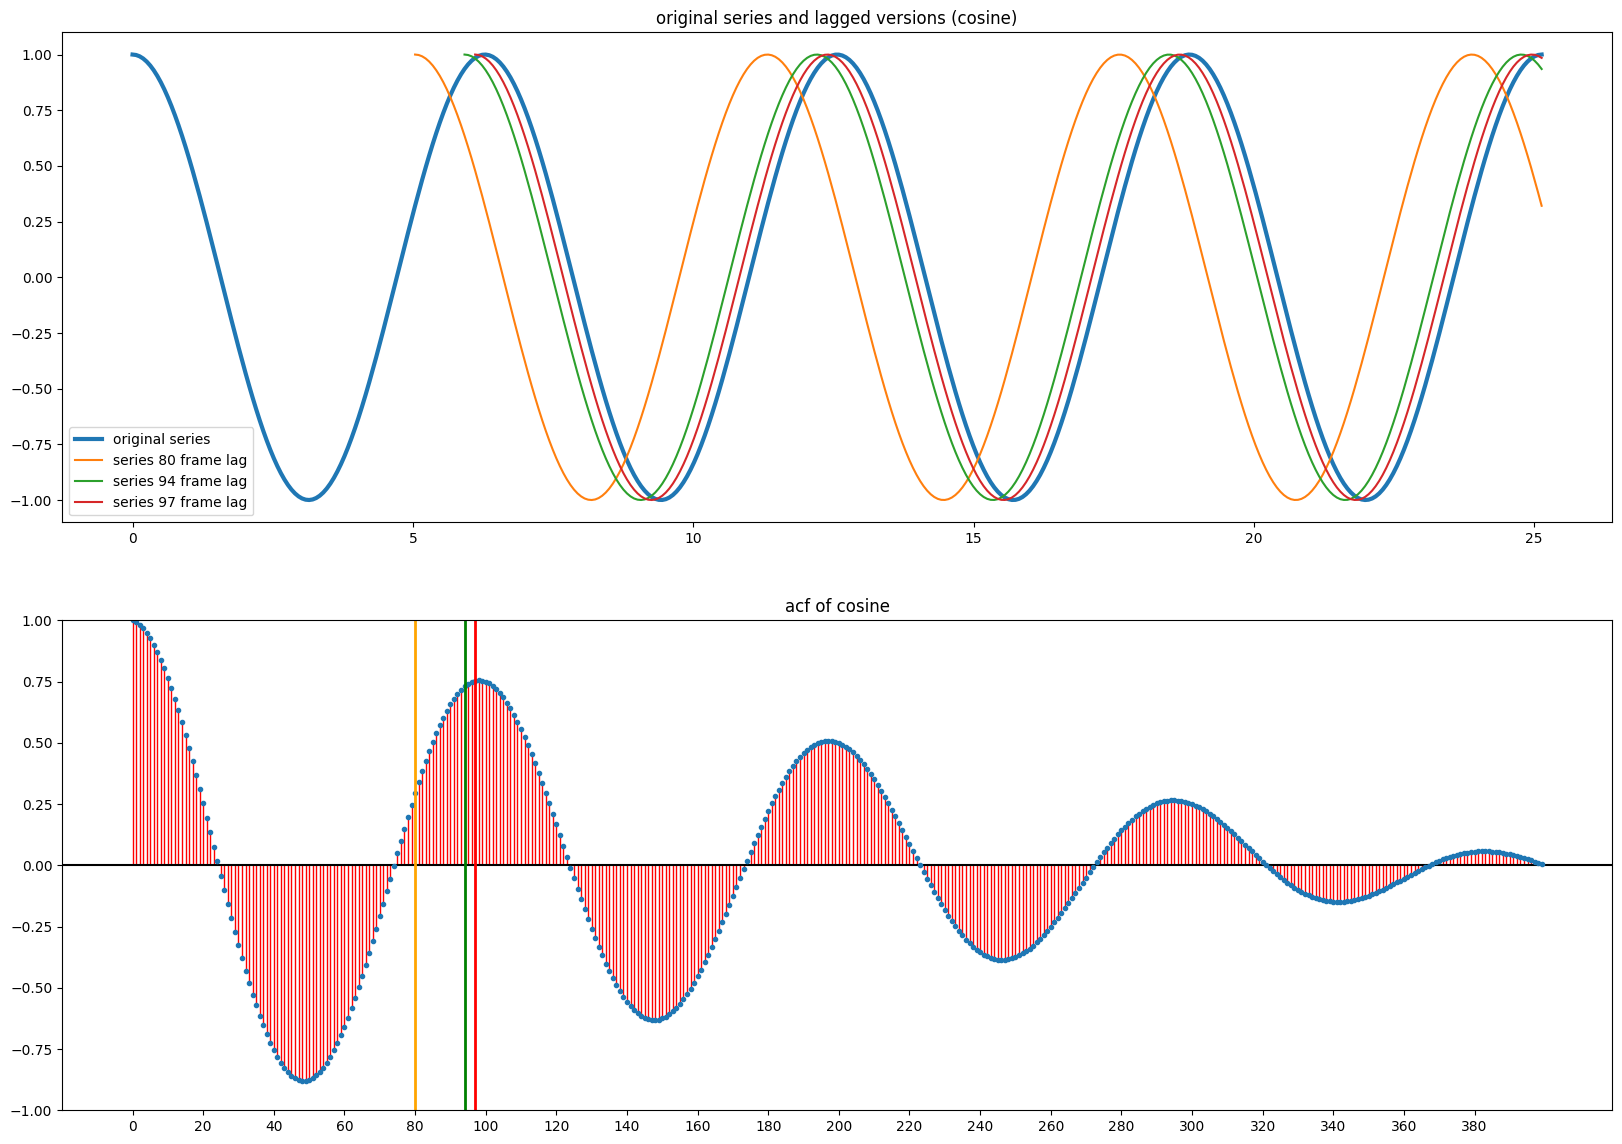
\includegraphics[width=\linewidth,keepaspectratio]{acf_cosine.png}
    \caption{Grafico di un coseno con sue versioni shiftate ed autocorrelazione.}
    \label{fig:acf_cosine}
\end{figure}
\begin{figure}[H]
    \centering
    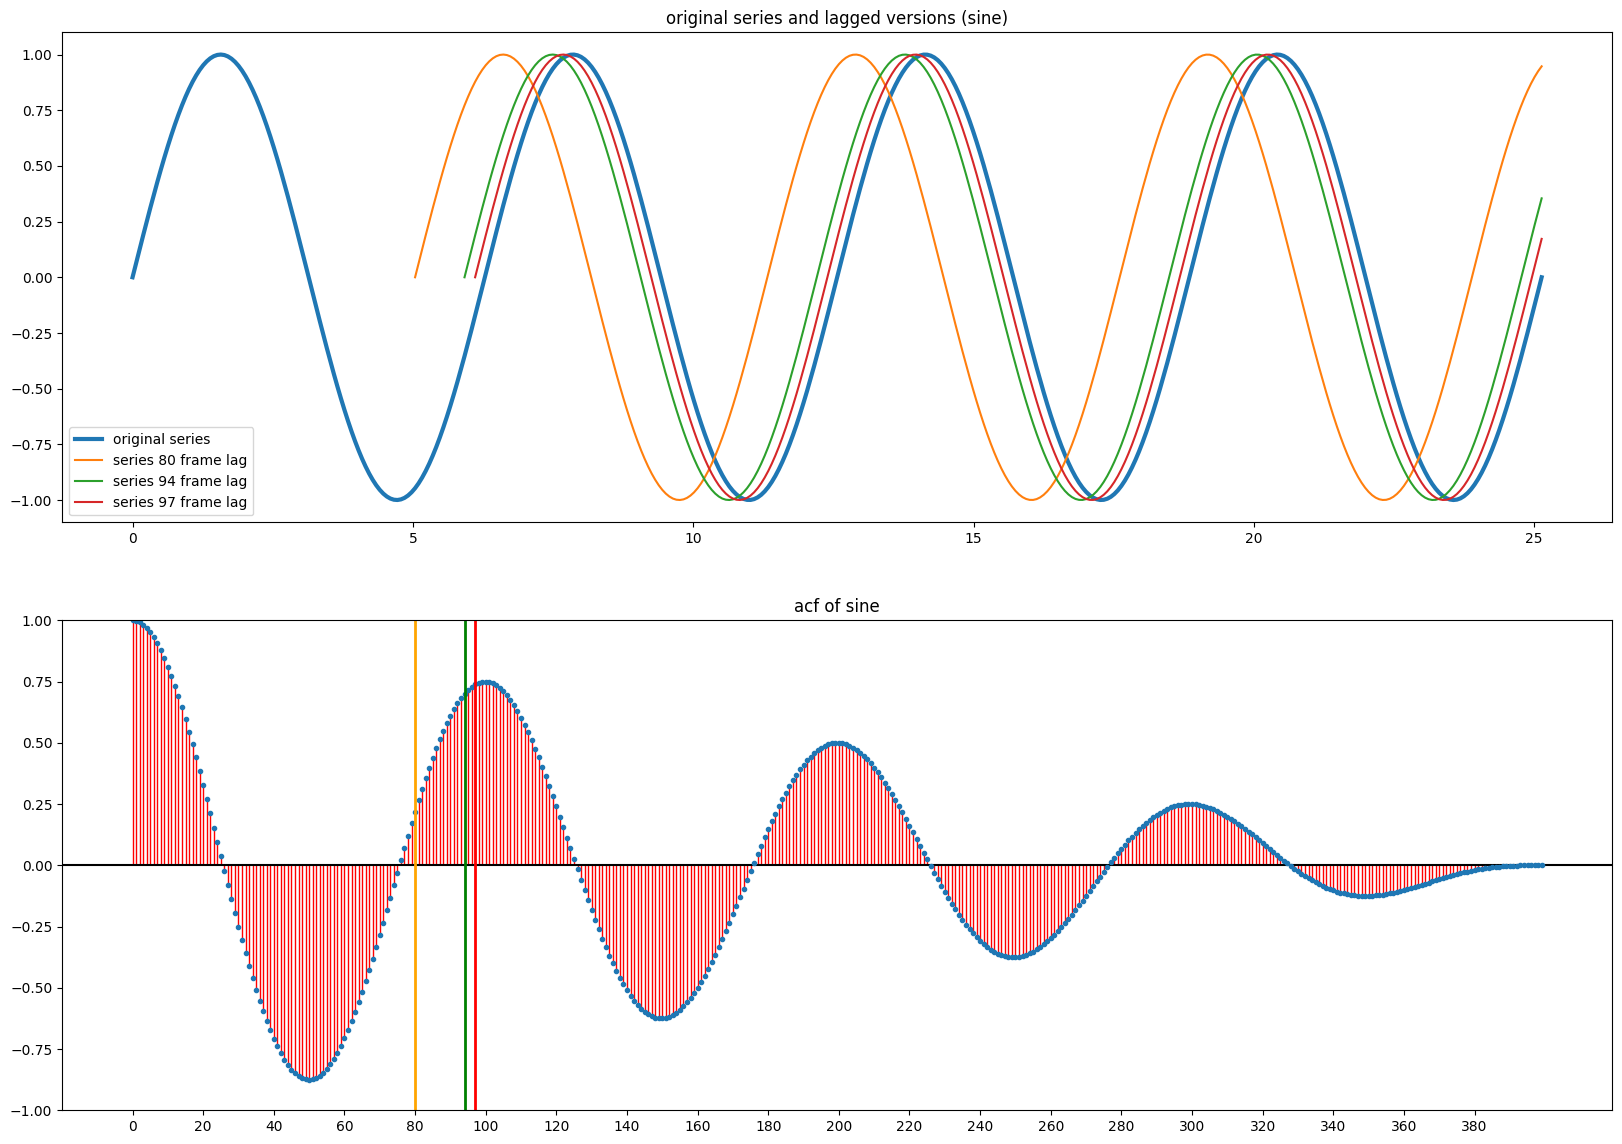
\includegraphics[width=\linewidth,keepaspectratio]{acf_sine.png}
    \caption{Grafico di un seno con sue versioni shiftate ed autocorrelazione.}
    \label{fig:acf_sine}
\end{figure}

Come possiamo vedere dai grafici in figura~\ref{fig:acf_cosine} e~\ref{fig:acf_sine} 
possiamo pensiamo al passo di una persona come un seno oppre ad un coseno. L'idea di utilizzare la
funzione di autocorrelazione nasce dal fatto che quando iniziamo a shiftare la serie
ed iniziamo a sovrapporre i passi, cioè quando le sinusoidi inizieranno ad allinearsi,
la correlazione aumenterà trovando così il pattern di camminata e la durata di uno stride.

\begin{sloppypar}
L'effetto di tendenza a $0$, all'aumentare del numero di frame, nel grafico dell'autocorrelazione,
è dovuto alla funzione di shift, quest'ultima per poter ``spostare'' la serie aggiunge degli $0$
a destra o a sinistra dipendentemente dal verso in cui si vuole eseguire lo shift.
\end{sloppypar}


Per dare un esempio più pratico prendiamo un sottoinseieme della serie relativa al piede 
destro posizione $1$ del soggetto sano $8$.

\begin{figure}[H]
    \centering
    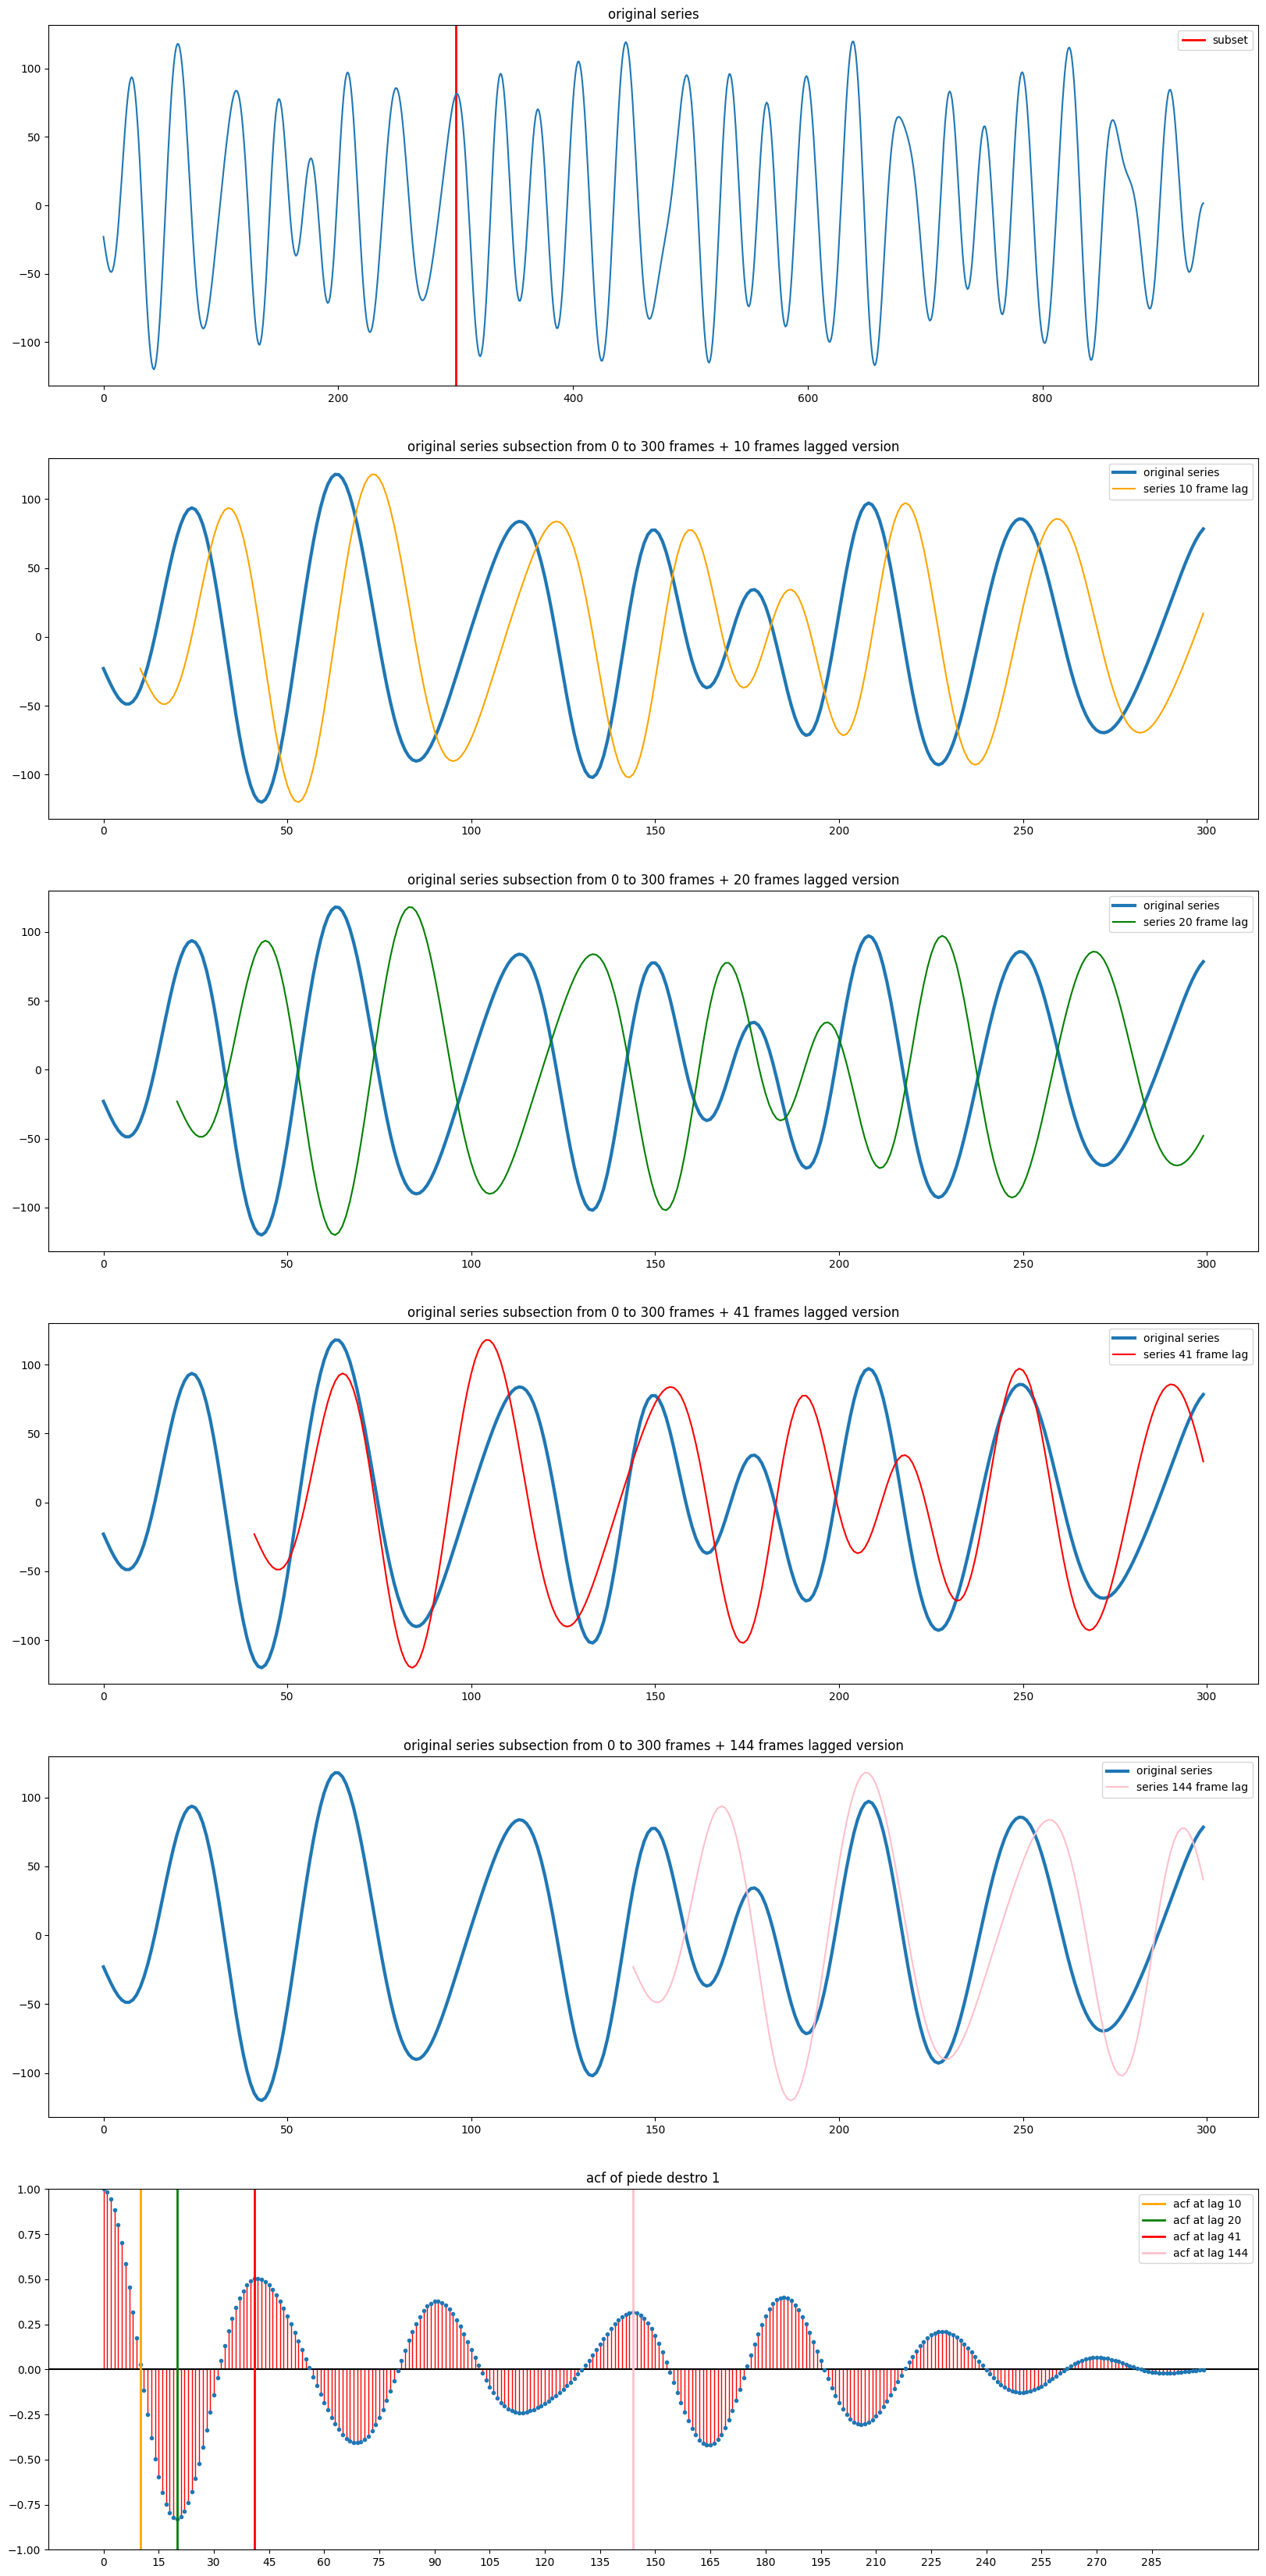
\includegraphics[width=0.8\linewidth,keepaspectratio]{acf_subset_x_piede_dx_008.png}
    \caption{Autocorrelazione con esempi di segnale shiftato.}
    \label{fig:acf_subset_x_piede_dx_008}
\end{figure}
In figura~\ref{fig:acf_subset_x_piede_dx_008} possiamo travere diversi grafici relativi alla
serie del paziente indicato sopra. Spieghiamo ora il loro significato:
\begin{enumerate}
    \item \textbf{Grafico in 1° posizione}: rappresenta la serie originale con una linea rossa (frame $300$)
    che indica il frame finale del sottoinsieme considerato dai grafici sottostanti.
    \item \textbf{Grafico in 2° posizione}:in blu viene rappresento il sottoinsieme preso in considerazione,
    cioè dal frame $0$ al $300$, ed in arancione lo stesso sottoinsieme ma shiftato di $10$ frame/lag.
    \item \textbf{Grafico in 3° posizione}: in blu viene rappresento il sottoinsieme preso in considerazione,
    cioè dal frame $0$ al $300$, ed in verde lo stesso sottoinsieme ma shiftato di $20$ frame/lag.
    \item \textbf{Grafico in 4° posizione}: in blu viene rappresento il sottoinsieme preso in considerazione,
    cioè dal frame $0$ al $300$, ed in rosso lo stesso sottoinsieme ma shiftato di $41$ frame/lag.
    \item \textbf{Grafico in 5° posizione}: in blu viene rappresento il sottoinsieme preso in considerazione,
    cioè dal frame $0$ al $300$, ed in rosa lo stesso sottoinsieme ma shiftato di $144$ frame/lag.
    \item \textbf{Grafico in 6° posizione}: la funzione di autocorrelazione calcolata su tutti i 
    lag possibili con linee di colore arancione, verde, rosso e rosa in prossimità dei valori 
    relativi alla correlazione tra la serie originale e la serie shiftata di $10$, $20$,
    $41$ e $144$ lag (in sostanza sono i valori delle correlazioni relative ai grafici $2$, $3$, $4$ e $5$).
\end{enumerate}

Possiamo notare che il primo valore della funzione di autocorrelazione, cioè il valore della correlazione
tra la seire originale e se stessa, è uguale ad $1$, di logica la massima correlazione possibile si può
avere quando la serie è perfettamente allineata con se stessa.

La correlazione tra la serie originale e la sua versione shiftata di $10$ lag invece ha valore
quasi uguale a $0$, questo perchè se si guarda il grafico numero $2$ in figura, la serie 
original e la sua versione shiftata in colore arancione si ``annullano'' avendo così correlazione
nulla. In altre parole quando la correlazione è vicina a $0$ la serie con la sua versione shiftata
sono ``molto'' diverse.

La correlazione tra la serie originale e la sua versione shiftata di $20$ lag ha un'alta correlazione
ma negativa, infatti se guardiamo il grafico numero $3$ possiamo vedere come la serie originale in blu
e la sua versione shiftata in verde sono una ``l'opposto'' dell'altra trovando così un'alta correlazione
ma negativa. Per poter immaginare una correlazione negativa possiamo pensare alla correlazione della serie
originale con una sua versione ribaltata sull'asse delle ascisse (in sostanza se $y$ è la nostra serie consideriamo $-y$),
il valore della correlazione a lag $0$ varrà $-1$.

Infine se consideriamo la correlazione tra la serie originale e la sua versione shiftata di $41$ lag
essa avrà un valore positivo ma ovviamente non $1$, se guardiamo il grafico numero $4$ possiamo notare
come la serie originale in blu e la serie shiftata in rosso tendano ad allinearsi, avendo così
come risultato una correlazione positiva.

Capito ora come poter interpretare la funzione di autocorrelazione relativa ad una serie 
continuiamo con l'implementazione della soluzione proposta.

\begin{sloppypar}
Utilizzando la funzione \texttt{argrelextrema} del modulo \texttt{statsmodels.tsa.stattools}
all'output della funzione di autocorrelazione è stato possibile recuperare gli argomenti (indici della lista) dei massimi locali.
Per esempio se prendiamo in considerazione il grafico~\ref{fig:P006_x_piede_dx_1_acf} gli argomenti
dei massimi locali sono
\end{sloppypar}
\[ [45, 95, 152, 197, 245, 297, 347, 395, 454, 504, 549, 592, 636, 678] \]
dove ogni argomento fa riferimento all'istante di tempo $t$, quindi al frame, in cui uno stride si ripete.

\begin{sloppypar}
Questo ovviamente succede in linea teorica, non sempre è detto che il grafico dell'autocorrelazione
riesca ad ottenere con precisione quest'informazione, soprattutto se i dati non sono filtrati correttamente.
\end{sloppypar}

Continuado con l'implementazione del metodo, calcolando la distanza tra un argomento e l'altro troveremo
la durata di quel determinato passo. Prendendo sempre in considerazione la lista di agromenti sopra
e calcolandone la prima differenza otterremo
\[[50, 57, 45, 48, 52, 50, 48, 59, 50, 45, 43, 44, 42]\]
dove ogni elemento rappresenta la durata di un singolo stride.

Se calcoliamo la media otterremo la durata media di uno stride, che per la lista sopra sarà di 
$48.69\texttt{frame}$ cioè $1.623\texttt{secondi}$.


\paragraph{Snippet} (\textit{Metodo per il calcolo dello stride})
\begin{minted}{python3}
    def stride(serie: list | np.ndarray):
        """ Calcola la durata di uno stride
            assumendo che la serie sia stazionaria    
        """

        # redi la serie un array numpy
        if not isinstance(serie, np.ndarray):
            serie = np.array(serie)
        
        # funzione di autocorrelazione
        acf = funzione_autocorrelazione(serie)

        # prende gli argomenti massimi locali della acf
        arg_max_locali = argrelextrema(acf, np.greater)[0]

        # differenza tra gli argomenti massimi locali
        arg_max_locali_diff = compute_first_diff(arg_max_locali)

        # calcola durata media di uno stride
        media_stride = arg_max_locali_diff.mean()

        if not isinstance(serie, np.ndarray):
            arg_max_locali_diff = arg_max_locali_diff.tolist()

        return arg_max_locali_diff, media_stride

\end{minted}


Questa serie di metodi è stata successivamente applicata ad ogni dataset ottenendo così la durata
media di uno stride per ogni posizione del piede destro e sinistro. Per fare ciò è stato creato
un ``mini'' programma che esegue automaticamente queste istruzioni ad ogni serie.

\subsubsection{Analisi di complessità}
\begin{sloppypar}
Assumendo che la serie fornita sia già stazionaria la complessità di questo algoritmo 
deriva pricipalmente dalla complessità della funzione \texttt{funzione\_autocorrelazione} e dalla complessità
della funzione \texttt{singola\_autocorrelazione} utilizzata dalla funzione di autocorrelazione.

Se consideriamo $n$ come la lunghezza della serie, 
la funzione \texttt{autocorrelazione\_singola} ha complessità temporale e spaziale $O(n)$ quindi
la funzione \texttt{funzione\_autocorrelazione} avrà complessità temporale $O(n^2)$ e complessità
spaziale $O(n)$.
\end{sloppypar}


\subsubsection{Analisi dei risultati e Conclusioni}
Per seplicità, i risultati verranno analizzati considerano un passo completo, cioè la somma degli stride
del piede destro e sinistro. Per fare chiarezza mostriamo un'immagine.
\begin{figure}[H]
    \centering
    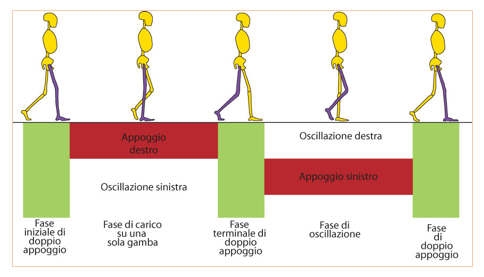
\includegraphics[width=0.8\linewidth,keepaspectratio]{passo_completo.png}
    \caption{Camminata di un soggetto~\cite{cf:passo_completo}.}
    \label{fig:passo_completo}
\end{figure}
Considerando la figura~\ref*{fig:passo_completo} stiamo valutando il periodo (durata) che parte dalla prima striscia
verde fino all'ultima striscia verde, quindi dall'inizio di una fase iniziale di doppio appoggio fino all'inzio
di un'altra fase iniziale di doppio appoggio.

\begin{sloppypar}
Detto ciò, compariamo ora la durata media dei passi completi dei soggetti sani e patologici. 

Si è trovato che la durata media di un passo completo con camminata normale è di rispettivamente $68,84 \ \texttt{frame}$
($2,294 \ \texttt{secondi}$) per i soggetti sani e di 
$81,71 \ \texttt{frame}$ ($2,723 \ \texttt{secondi}$) per i soggetti patologici.
I soggetti patologici, con camminata normale, hanno quindi una durata di passo completo maggiore del 
$19,84\%$ rispetto alla durata di un passo completo, con camminata normale, dei soggetti sani.
\end{sloppypar}

Applicando lo stesso ragionamento alle camminata tacco-punta e punta si è riscontrato che 
i soggetti patologici, con camminata tacco-punta, hanno una durata di passo completo maggiore del 
$8.28\%$ rispetto alla durata di un passo completo, con camminata tacco-punta, dei soggetti sani, 
mentre nella camminata punta si è riscontrata una durata maggiore del $43,04\%$.

I risultati ottenuti analizzando i dati delle camminate tacco-punta e punta non possono ritenersi affidabili
in quanto le percentuali e le medie sono state calcolate con troppe poche osservazioni.


\paragraph*{Premessa sui risultati}
I risultati sopra ottenuti non sono da prendere come riferimento in quanto essi sono ottenuti
mediante l'ausilio di un metodo non totalmente sicuro. Il metodo utilizzato è sperimentale e tantomeno 
fine allo scopo del tirocinio quindi potrebbe giungere a risultati non corretti 
poiché la funzione di autocorrelazione potrebbe rilevare pattern e correlazioni diverse da quelle
aspettate ed anche perché questa tecnica è stata applicata a serie filtrate in un certo modo.

\paragraph*{Problemi non totalmente risolti o ancora incogniti}
Una incognita rimasta aperta dopo l'analisi dei grafici dell'autocorrelazione e delle serie originali
è l'effetiva importanza in questa soluzione di rendere le serie stazionarie. 
La funzione di test Dickey-Fuller per l'analisi della stazionarietà fornita dal 
pacchetto \texttt{statsmodels} ha la possibilità
di capire automaticamente il numero di lag su cui eseguire il test e, per come è stato implementata
la soluzione, l'algoritmo rileva un numero di lag non sufficiente per ottenere un risultato 
di test veritiero.

Considerato il fatto che la funzione della soluzione che rende le serie stazionarie non 
rileva propriamente quando una serie è stazionaria, e quindi tutte le analisi successive
sono state eseguite su serie non propriamente stazionarie, i risultati ottenuti non sono
si discostano molto dalla realtà. Questo potrebbe essere dovuto a come sono stati
filtrati i dati in partenza, e quindi, per questa determinata applicazione, non è stato necessario 
avere delle serie propriamente stazionarie.

In breve con lo sviluppo di questa soluzione e l'interpretazione dei risultati ottenuti
non si è riuscita a cogliere l'importanza di avere una serie stazionaria non trovando
molta differenza tra una serie stazionaria ed una non stazionaria (sempre rimanendo nei
limiti di quest'applicazione).

\subsection{Seconda Soluzione}
In questa sezione verrà mostrata la seconda soluzione al problema posto, nello
specifico verrà spiegata in breve l’idea generale, l’implementazione di alcune parti relative all'algoritmo, 
l’analisi dei risultati, l’analisi della complessità ed infine
le conclusioni.

\subsubsection{Idea generale}
In questa soluzione al problema si è pensato di considerare la scoposizione delle serie nelle 
loro componenti quali trend, stagionalità e residui. Nello specifico l'idea è nata
pensado che possiamo considerare ad un passo (stride) di un soggetto come ad un evento periodico
che si ripete più o meno in ugual maniera nel tempo ad uno specifico periodo. Considerando quindi
la scoposizione nelle tre compnenti di una serie, la stagionaità ad un determinato periodo potrebbe
rappresentare l'informazione che stiamo cercando di ottenere. Questo avviene solamente il linea teorica
in quanto non è detto che il passo di un soggetto avvenga sempre ad intervalli precisi ma l'idea è che
ad un certo periodo la stagionalità raccolga la maggior parte dell'informazione cercata.

Essendo che questo processo si può provare attuare solamente guardando il grafico della stagionalità
si è pensato di automatizzarlo cercando un algoritmo che, data una serie temporare relativa ad un giunto,
esso dia come risultato un periodo
la cui stagionaità raccolga la maggior parte dell'informazione di un passo. Per fare ciò è stato 
necessario comparare due serie, o meglio detto, è stato necessario comparare la serie relativa 
ad un giunto divisa a metà considerando le due metà come serie separate. Successivamente
si è calcolata la stagionalità su più periodi per entrambe le serie. In linea teorica i periodi con
stagionalità simili sarebbero dovute essere i pattern che occorrono in entrambe le serie,
mentre le stagionalità ``diverse'' sarebbero dovute essere pattern che non rientrano 
in entrambe probabilmente dovuto ad altre motivazioni quali, ad esempio, del rumore ancora presente.





\subsubsection{Implementazione}
Per prima cosa è necessario dividere una serie relativa ad un giunto di un soggetto in due e decidere
su quali periodi calcolare la stagionalità.

\begin{sloppypar}
Successivamente per ogni periodo si è calcolata la stagionalità delle due parti
calcolandone la differenza quindi l'errore tra le due stagionalità. Per calcolare la stagionalità
è stata utilizzata la funzione \texttt{seasonal\_decompose} del modulo \texttt{statsmodels.tsa.seasonal}
relativo al pacchetto \texttt{statsmodels}, mentre per il calcolo dell'errore
le due stagionalità sono state convertite nel dominio delle frequenze, utilizzando la trasformata
di Fourier, e calcolata la differenza di ampiezza tra frequenze. L'algoritmo è stato 
creato per poter accettare anche serie divise in più di due parti.
\end{sloppypar}

Vediamo ora come è stata implementata la funzione che esegue il calcolo dell'errore.

\paragraph*{Snippet} (\textit{Calcolo dell'errore tra stagionalità})
\begin{minted}{python3}
    def freq_error(season_1: list, season_2: list):

        # prendi la lunghezza minima 
        min_len = 0
        if len(season_1) < len(season_2):
            min_len = len(season_1)
        else:
            min_len = len(season_2)

        # calcolo della trasformata di 
        # Fourier tra stagionalità
        fft_season_1 = sft.fft(season_1, min_len)
        fft_season_2 = sft.fft(season_2, min_len)

        # calcolo del magnitudo per ogni trasformata
        fft_season_1_m = np.abs(fft_season_1) / len(season_1)
        fft_season_2_m = np.abs(fft_season_2) / len(season_2)

        # differenza tra frequenze
        fft_diff = []
        for idx in range(min_len//2):
            fft_diff.append(fft_season_1_m[idx] - fft_season_2_m[idx])
        
        # calcolo dell'errore quadratico medio
        return np.power(fft_diff, 2).mean() 
\end{minted}


Vediamo ora il metodo principale.
\paragraph*{Snippet} (\textit{Metodo per la soluzione al problema (2)})
\begin{minted}{python3}
    def soluzione_2(seriesList, periods):
        """ 
        seriesList = 
                lista che contiene la serie divisa in due parti
                quindi due liste

        periods = 
                lista di interi, è la lista che
                contiene i periodi su cui calcolare
                la stagionalità
        """
        # per ogni periodo
        errors = []
        for j, period in enumerate(periods):

            # non è possibile calcolare 
            # la stagionalità per il periodo 0
            if period == 0:
                raise Exception('stagionalità non calcolabile \
                    con periodo 0')

            # calcola l'errore le parti della serie
            aux_errors = []
            for idx, series in enumerate(seriesList):

                # stagionalità della prima parte
                season = seasonal_decompose(
                    series, period=period).seasonal

                
                for idx in range(idx+1, len(seriesList)):

                    # stagionalità della seconda parte 
                    # (e altre parti)
                    aux_season = seasonal_decompose(
                        seriesList[idx], period=period).seasonal
                    
                    # calcolo dell'errore tra stagionalità
                    aux_errors.append(
                        freq_error(season, aux_season)
                    )
            

            errors.append(np.mean(aux_errors))

        return np.min(errors), periods[np.argmin(errors)], errors
\end{minted}

Come possiamo vedere dall'implementazione come risultato otteniamo l'errore minimo, il periodo
associato all'errore minimo e la lista contenente, per ogni periodo, l'errore associato.

In una fase successiva è stata creata una funzione che permette di analizzare la lista relativa
agli errori per ogni periodo creando dei grafici che indicano i periodi ``salienti''. 
L'implementazione di quet'ultima non verrà data ma il concetto è che per periodi piccoli l'errore
è sempre il minimo e crescente e, dopo un certo periodo, l'errore inizia ad aumentare drasticamente
per poi diminuire successivamente dopo aver trovato una stagionalià nuovamente simile tra le due serie.
Per capire meglio consideriamo la lista degli errori tra $1$ e $30$, in questo range l'errore è crescente
per ogni periodo, dal periodo $31$ in poi l'errore aumenta drasticamente fino al periodo $80$ per poi diminuire
nuovamente ed ad un certo punto riaumentare. Questo è dovuto appunto al fatto che quando le stagionalità non si
``assomigliano'' l'errore sarà alto mentre per stagionalità simili l'errore è minimo o comunque molto basso.

\subsubsection{Analisi di complessità}
Consideriamo come $m$ il numero di sottoinsiemi, di ugual lunghezza, creati a partire da una serie 
(negli esempi sopra abbiamo sempre considerato di dividere la serie in due parti),
$n$ la lunghezza di un sottoinsieme, $S$ la complessità della 
funzione \texttt{seasonal\_decompose} e tenuto conto che il periodo massimo su cui è possibile
calcolare quest'ultima è di $(m/2)$, la complessità temporale della seconda soluzione è 
$O( (n/2)m\log{(m)}Sn\log{(n)} )$ mentre la complessità spaziale sarà $O( n+2n+(n/2) )$ quindi $O(n)$.


\subsubsection{Analisi dei risultati e Conclusioni}
Analizziamo ora qualche grafico cercando di capire meglio come rappresentare i risultati del metodo
spiegato nella sezione precedente.
\begin{figure}[H]
    \centering
    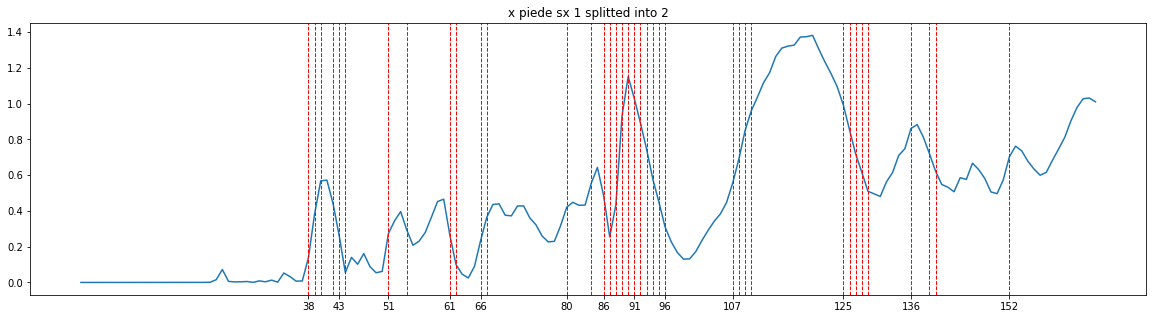
\includegraphics[width=0.8\linewidth,keepaspectratio]{x_piede_sx_1_006.png}
    \caption{Grafico degli errori per ogni periodo relativo al piede sinitro posizione 1 del soggetto patologico $6$.}
    \label{fig:x_piede_sx_1_006_m2}
\end{figure}
\begin{figure}[H]
    \centering
    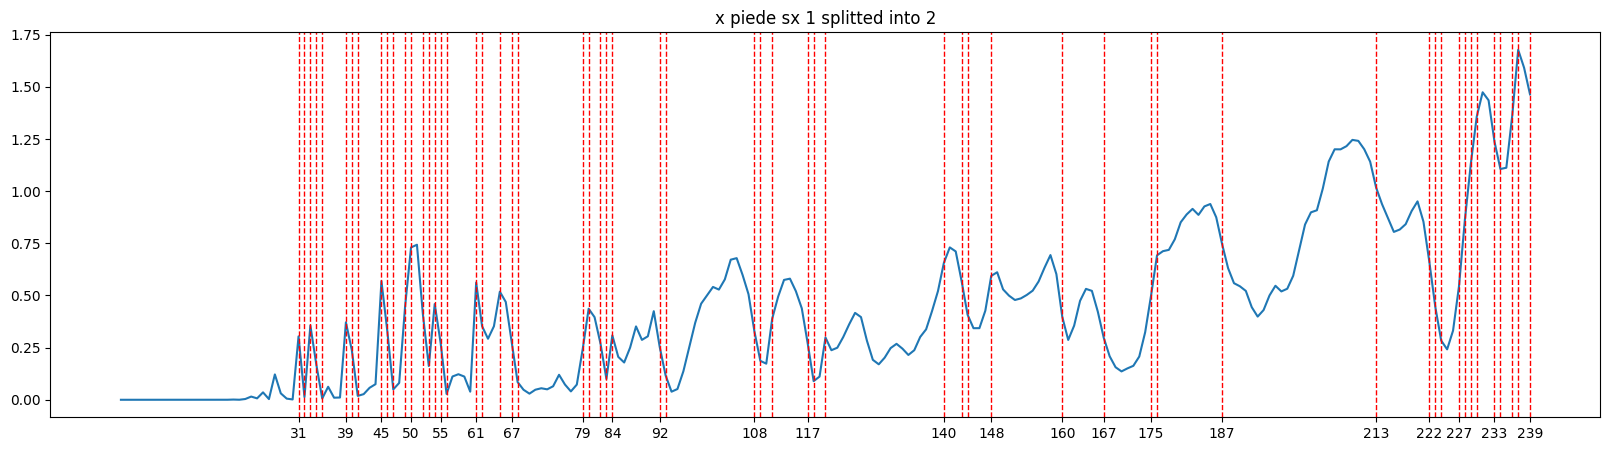
\includegraphics[width=0.8\linewidth,keepaspectratio]{x_piede_sx_1_008.png}
    \caption{Grafico degli errori per ogni periodo relativo al piede sinitro posizione 1 del soggetto sano $8$.}
    \label{fig:x_piede_sx_1_008_m2}
\end{figure}
\begin{figure}[H]
    \centering
    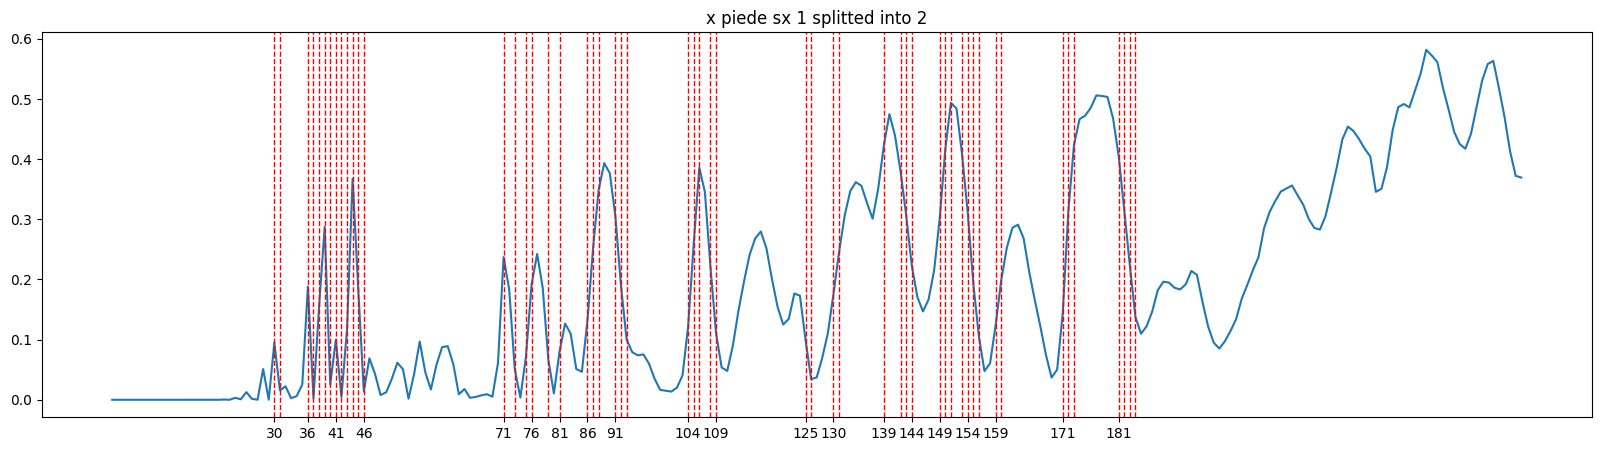
\includegraphics[width=0.8\linewidth,keepaspectratio]{x_piede_sx_1_021.png}
    \caption{Grafico degli errori per ogni periodo relativo al piede sinitro posizione 1 del soggetto patologico $21$.}
    \label{fig:x_piede_sx_1_021_m2}
\end{figure}

Nei grafici in figura~\ref*{fig:x_piede_sx_1_006_m2},~\ref*{fig:x_piede_sx_1_008_m2} e~\ref*{fig:x_piede_sx_1_021_m2}
sono rappresentati gli errori sull'asse delle ordinate ed i periodi, a cui ogni errore è associato,
sull'asse delle ascisse. Le linee rosse verticali rappresentano i punti salienti, calcolate mediante
l'asulio di una funzione che utilizza la media e deviazione standard della differenza tra un errore 
e quello successivo.

Controllando diversi grafici si è potuto notato che, per molte serie, in prossimità del periodo 
relativo ad un passo (stride) l'errore inizia ad alzarsi, in questo modo dovrebbe essere possibile 
calcolare la durata di un passo.
Questo però non succede sempre, con alcune serie questo fenomeno non si manifesta o comunque
si manifesta ma non in corrispondenza del periodo legato ad un passo, rendendo quindi impossibile
reperire l'informazione necessaria.

Questo potrebbe essere causato dal fatto che la funzione di seasonal decompose ``aggiusta'' la componente
di residui per riuscire ad ottenere una periodicità nella componente di stagionalità.

Tenendo a mente le considerazioni fatte fino questo punto possiamo quindi considerare i risultati ottenuti,
e di conseguenza questa soluzione, come non validi, essendo che non si ha la sicurezza di poter
ottenere risultati coerenti per la ricerca dell'informazione interessata.



\subsection{Conclusioni Finali}
Prendendo in considerazione la prima soluzione, spiegata nella sezione precedente, possiamo concludere
che la funzione di autocorrelazione può essere utilizzata per la soluzione a problemi di questa tipologia,
più in particolare essa può essere utilizzata per trovare pattern e/o caratteristiche presenti nei dati, 
che dal grafico potrebbero non essere evidenti.

La seconda soluzione proposta invece non è stata utile allo scopo di trovare un singolo passo 
relativo ad un soggetto. Normalmente consideriamo azioni abituali, come ad esempio il passo,
come pattern, di un determinato periodo, che si ripetono nel tempo quando invece nella realtà non 
è così. 
Tuttavia, l'algoritmo presentato nella seconda soluzione, potrebbe essere utilizzato 
in altre applicazioni la cui necessità ricade sul trovare periodi in cui occorrono stagionalità simili 
appartenenti a serie temporali diverse, oppure esso potrebbe essere preso come spunto implementativo per la creazione di un ulteriore 
algoritmo.

In conclusione, possiamo constatare che le tecniche utilizzate per l'analisi di serie temporali
possono essere d'aiuto per una prima analisi non accurata del problema,
non sostituendo però le tecniche tuttora utilizzate per analisi a problemi di questa tipologia.


